% Content for Chapter 5, Section 5.7 — pulled in by chapters/05-system-design.tex
\subsection{مكوّنات الخدمة}

هي الخدمة الوحيدة في النظام التي لا تملك قاعدة بيانات ولا واجهة \en{HTTP} واردة، فهي مستهلِكة صرفة. ويعرض الشكل~\ref{fig:comp-04} مكوّناتها.

\begin{figure}[htbp]
  \centering
  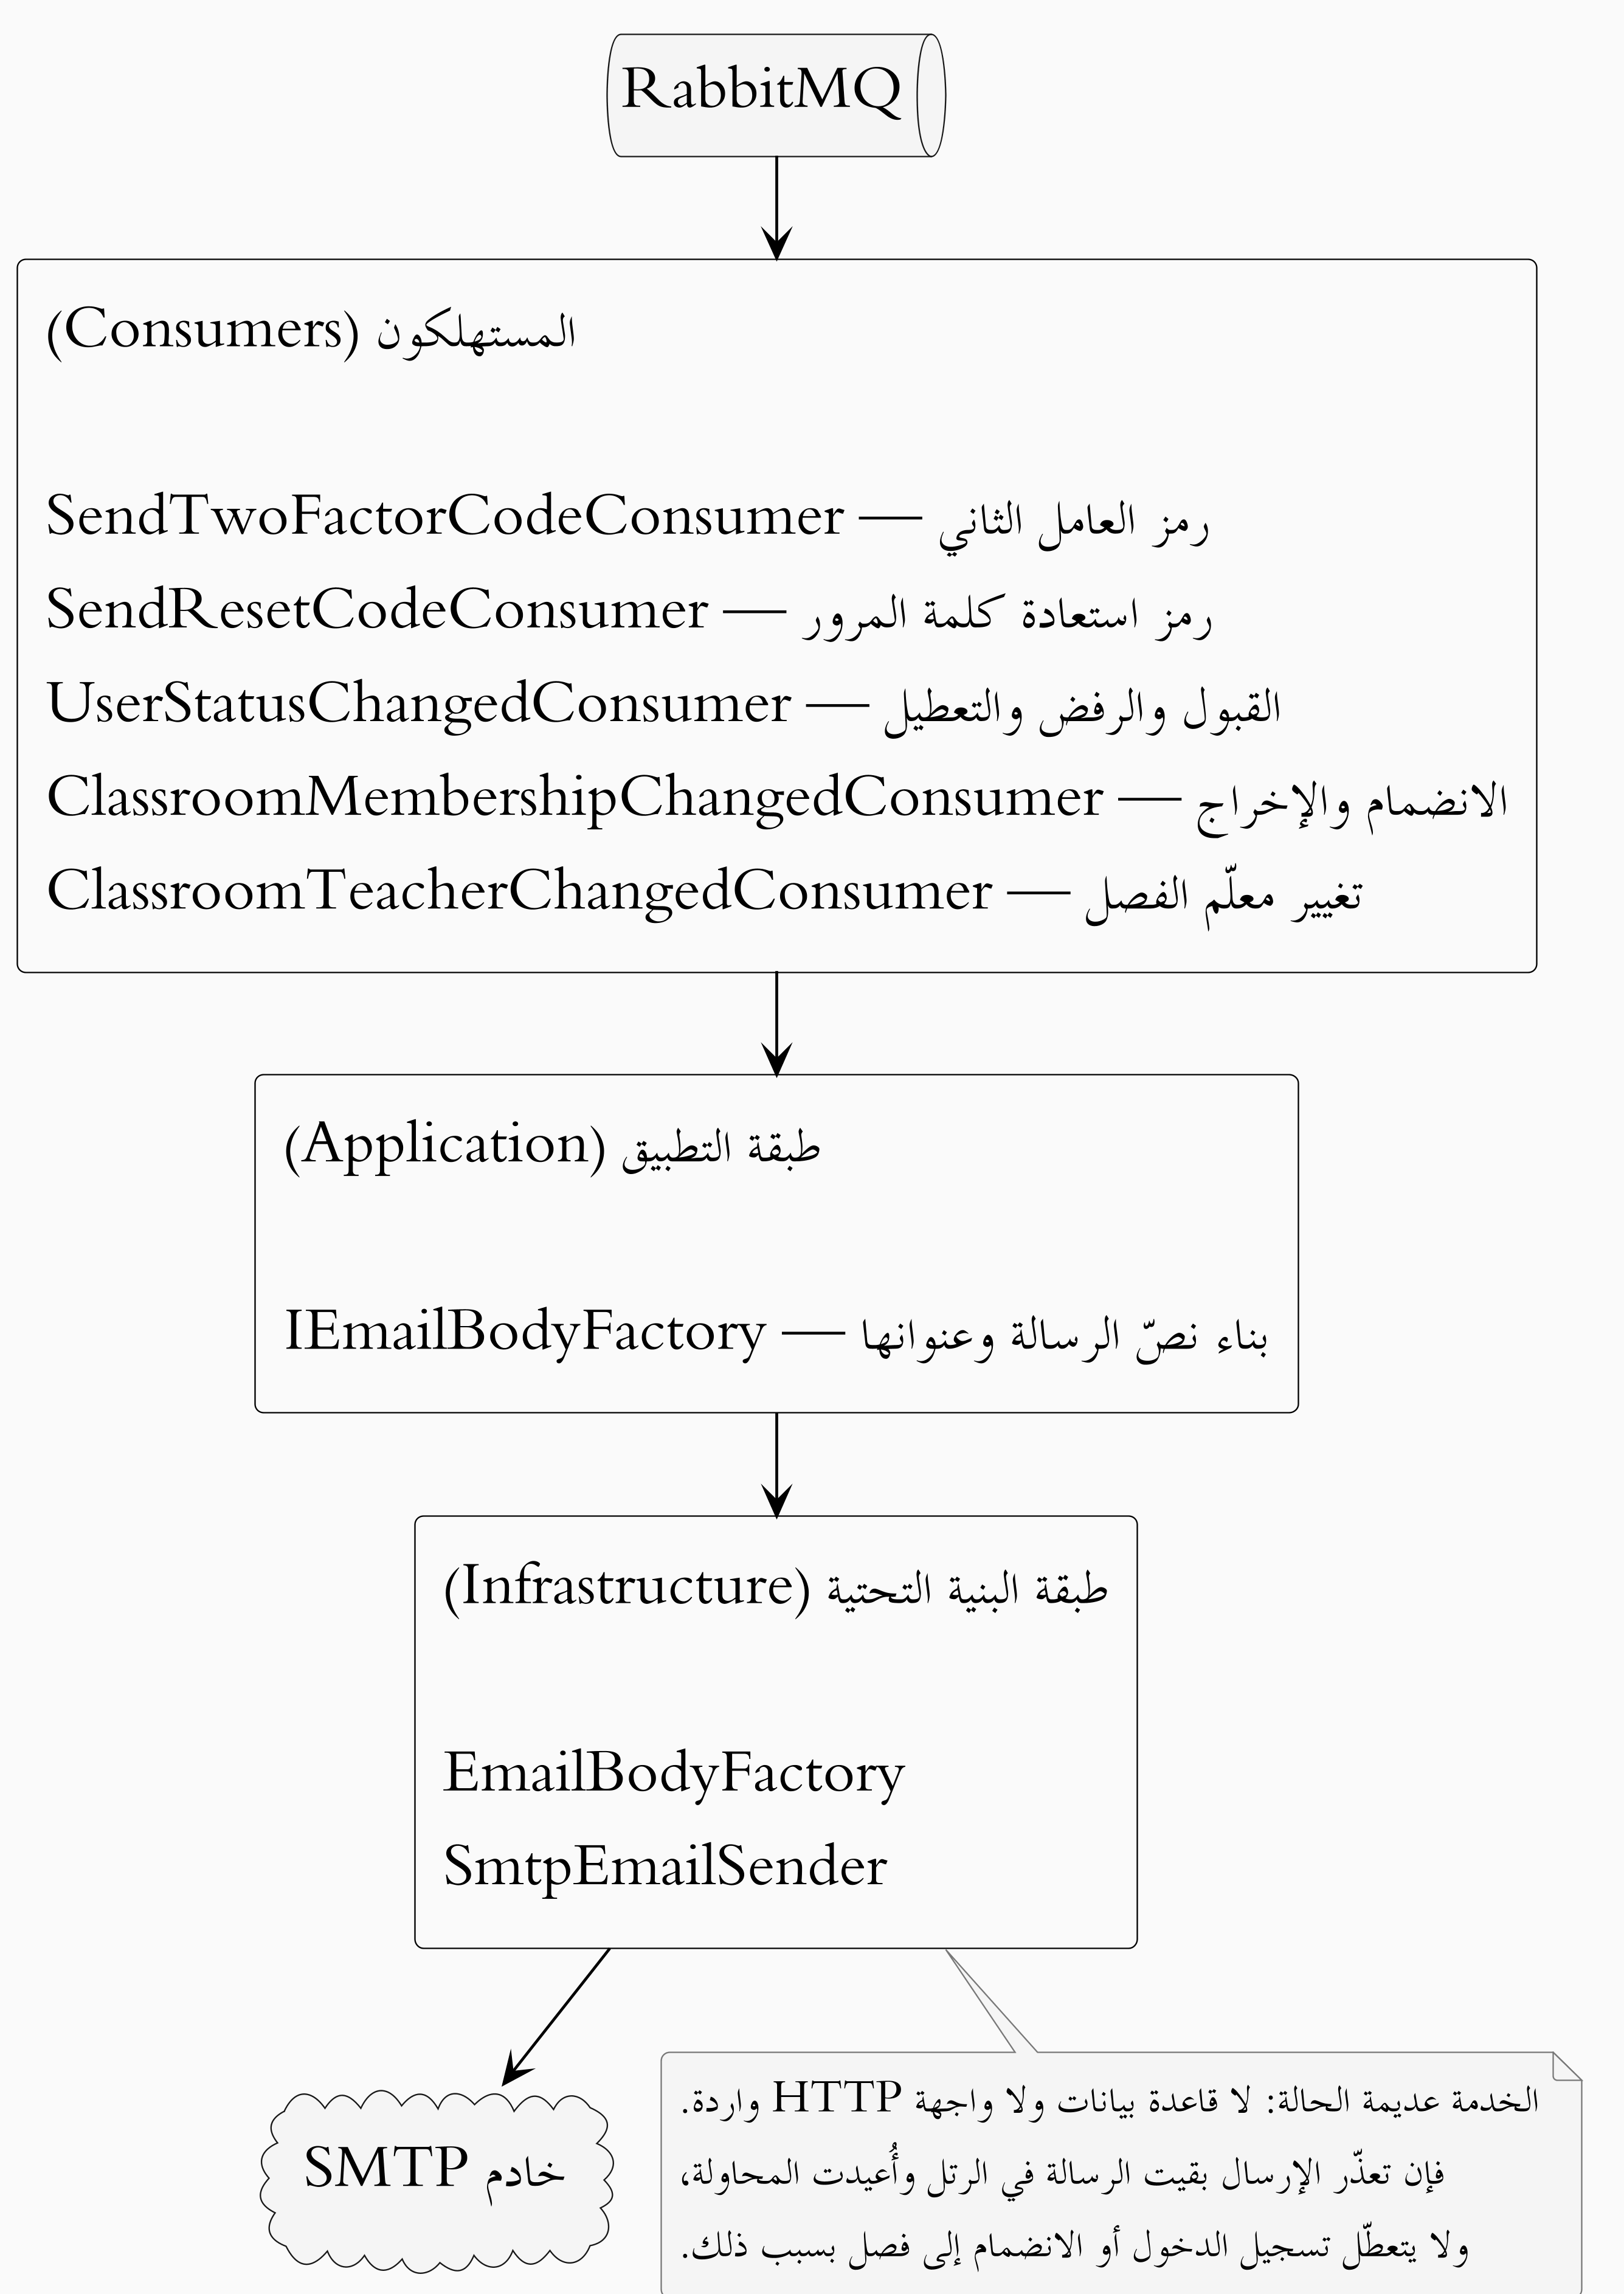
\includegraphics[width=\textwidth,height=0.8\textheight,keepaspectratio]{figures/comp-04-email.png}
  \caption{مخطط المكوّنات التفصيلي لخدمة البريد.}
  \label{fig:comp-04}
\end{figure}

ويُبيَّن مسار الإشعار من لحظة نشره إلى لحظة تسليمه، وما يحقّقه من فكِّ الارتباط الزمني، في القسم~\ref{subsubsec:flow-email}.
